\documentclass{standalone}
\usepackage{tikz}
\usetikzlibrary{patterns, positioning}

\begin{document}
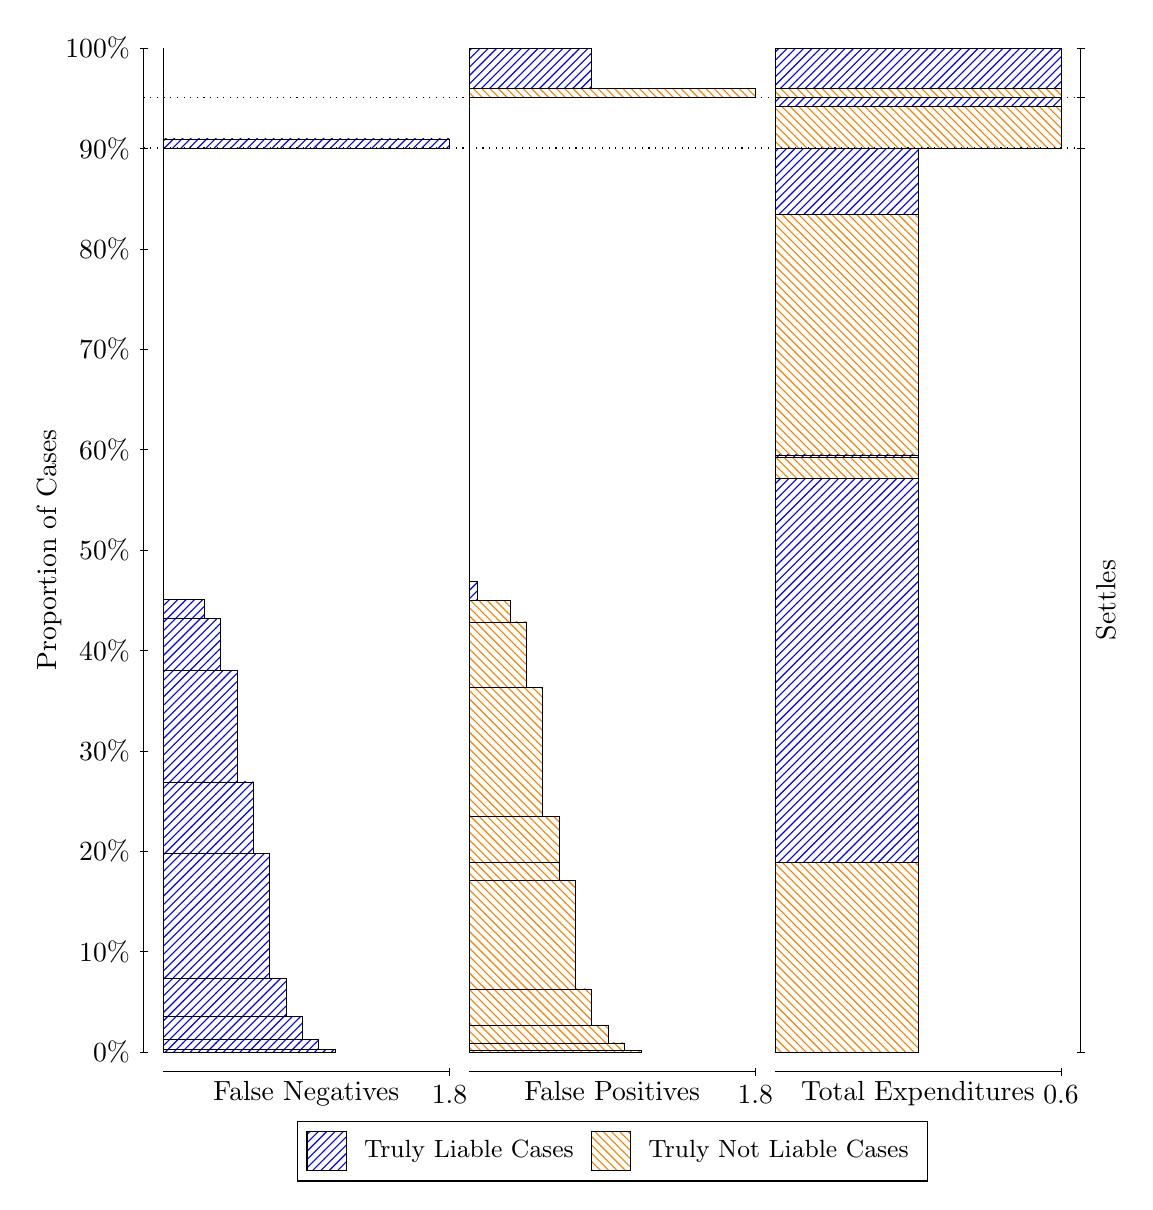
\begin{tikzpicture}
\draw[black, very thin] (1.5,1.75) -- (1.5,14.5);
\node[rotate=90, anchor=center] at (0.3, 8.125) {Proportion of Cases};
\draw[black, very thin] (1.45,1.75) -- (1.55,1.75);
\node[anchor=east] at (1.45, 1.75) {0\%};
\draw[black, very thin] (1.45,3.025) -- (1.55,3.025);
\node[anchor=east] at (1.45, 3.025) {10\%};
\draw[black, very thin] (1.45,4.3) -- (1.55,4.3);
\node[anchor=east] at (1.45, 4.3) {20\%};
\draw[black, very thin] (1.45,5.575) -- (1.55,5.575);
\node[anchor=east] at (1.45, 5.575) {30\%};
\draw[black, very thin] (1.45,6.85) -- (1.55,6.85);
\node[anchor=east] at (1.45, 6.85) {40\%};
\draw[black, very thin] (1.45,8.125) -- (1.55,8.125);
\node[anchor=east] at (1.45, 8.125) {50\%};
\draw[black, very thin] (1.45,9.4) -- (1.55,9.4);
\node[anchor=east] at (1.45, 9.4) {60\%};
\draw[black, very thin] (1.45,10.675) -- (1.55,10.675);
\node[anchor=east] at (1.45, 10.675) {70\%};
\draw[black, very thin] (1.45,11.95) -- (1.55,11.95);
\node[anchor=east] at (1.45, 11.95) {80\%};
\draw[black, very thin] (1.45,13.225) -- (1.55,13.225);
\node[anchor=east] at (1.45, 13.225) {90\%};
\draw[black, very thin] (1.45,14.5) -- (1.55,14.5);
\node[anchor=east] at (1.45, 14.5) {100\%};

\draw[black, very thin] (13.4,1.75) -- (13.4,14.5);
\draw[black, very thin] (13.35,1.75) -- (13.45,1.75);
\node[anchor=west] at (13.35, 1.75) {};
\draw[black, very thin] (13.35,13.23) -- (13.45,13.23);
\node[anchor=west] at (13.35, 13.23) {};
\draw[black, very thin] (13.35,13.87) -- (13.45,13.87);
\node[anchor=west] at (13.35, 13.87) {};
\draw[black, very thin] (13.35,14.5) -- (13.45,14.5);
\node[anchor=west] at (13.35, 14.5) {};

\draw[black, very thin, pattern color=blue, pattern=north east lines] (1.75,1.75) rectangle (3.93,1.7782);
\draw[black, very thin, pattern color=blue, pattern=north east lines] (1.75,1.7782) rectangle (3.7224,1.9068);
\draw[black, very thin, pattern color=blue, pattern=north east lines] (1.75,1.9068) rectangle (3.5148,2.2049);
\draw[black, very thin, pattern color=blue, pattern=north east lines] (1.75,2.2049) rectangle (3.3071,2.6825);
\draw[black, very thin, pattern color=blue, pattern=north east lines] (1.75,2.6825) rectangle (3.0995,4.2758);
\draw[black, very thin, pattern color=blue, pattern=north east lines] (1.75,4.2758) rectangle (2.8919,5.1789);
\draw[black, very thin, pattern color=blue, pattern=north east lines] (1.75,5.1789) rectangle (2.6843,6.6002);
\draw[black, very thin, pattern color=blue, pattern=north east lines] (1.75,6.6002) rectangle (2.4767,7.2579);
\draw[black, very thin, pattern color=blue, pattern=north east lines] (1.75,7.2579) rectangle (2.269,7.4946);
\draw[black, very thin, pattern color=orange, pattern=north west lines] (1.75,7.4946) rectangle (1.75,13.23);
\draw[black, very thin, pattern color=blue, pattern=north east lines] (1.75,13.23) rectangle (5.3833,13.345);
\draw[black, very thin, pattern color=orange, pattern=north west lines] (1.75,13.345) rectangle (1.75,13.87);
\draw[black, very thin, pattern color=orange, pattern=north west lines] (1.75,13.87) rectangle (1.75,13.984);
\draw[black, very thin, pattern color=blue, pattern=north east lines] (1.75,13.984) rectangle (1.75,14.5);
\draw[black, very thin, pattern color=orange, pattern=north west lines] (5.6333,1.75) rectangle (7.8133,1.7745);
\draw[black, very thin, pattern color=orange, pattern=north west lines] (5.6333,1.7745) rectangle (7.6057,1.8657);
\draw[black, very thin, pattern color=orange, pattern=north west lines] (5.6333,1.8657) rectangle (7.3981,2.0875);
\draw[black, very thin, pattern color=orange, pattern=north west lines] (5.6333,2.0875) rectangle (7.1905,2.5509);
\draw[black, very thin, pattern color=orange, pattern=north west lines] (5.6333,2.5509) rectangle (6.9829,3.9244);
\draw[black, very thin, pattern color=orange, pattern=north west lines] (5.6333,3.9244) rectangle (6.7752,4.1573);
\draw[black, very thin, pattern color=orange, pattern=north west lines] (5.6333,4.1573) rectangle (6.7752,4.739);
\draw[black, very thin, pattern color=orange, pattern=north west lines] (5.6333,4.739) rectangle (6.5676,6.3779);
\draw[black, very thin, pattern color=orange, pattern=north west lines] (5.6333,6.3779) rectangle (6.36,7.2131);
\draw[black, very thin, pattern color=orange, pattern=north west lines] (5.6333,7.2131) rectangle (6.1524,7.4857);
\draw[black, very thin, pattern color=blue, pattern=north east lines] (5.6333,7.4857) rectangle (5.7371,7.7224);
\draw[black, very thin, pattern color=blue, pattern=north east lines] (5.6333,7.7224) rectangle (5.6333,13.23);
\draw[black, very thin, pattern color=orange, pattern=north west lines] (5.6333,13.23) rectangle (5.6333,13.755);
\draw[black, very thin, pattern color=blue, pattern=north east lines] (5.6333,13.755) rectangle (5.6333,13.87);
\draw[black, very thin, pattern color=orange, pattern=north west lines] (5.6333,13.87) rectangle (9.2667,13.984);
\draw[black, very thin, pattern color=blue, pattern=north east lines] (5.6333,13.984) rectangle (7.1905,14.5);
\draw[black, very thin, pattern color=orange, pattern=north west lines] (9.5167,1.75) rectangle (11.333,4.1573);
\draw[black, very thin, pattern color=blue, pattern=north east lines] (9.5167,4.1573) rectangle (11.333,9.0308);
\draw[black, very thin, pattern color=orange, pattern=north west lines] (9.5167,9.0308) rectangle (11.333,9.3035);
\draw[black, very thin, pattern color=blue, pattern=north east lines] (9.5167,9.3035) rectangle (11.333,9.3317);
\draw[black, very thin, pattern color=orange, pattern=north west lines] (9.5167,9.3317) rectangle (11.333,12.387);
\draw[black, very thin, pattern color=blue, pattern=north east lines] (9.5167,12.387) rectangle (11.333,13.23);
\draw[black, very thin, pattern color=orange, pattern=north west lines] (9.5167,13.23) rectangle (13.15,13.755);
\draw[black, very thin, pattern color=blue, pattern=north east lines] (9.5167,13.755) rectangle (13.15,13.87);
\draw[black, very thin, pattern color=orange, pattern=north west lines] (9.5167,13.87) rectangle (13.15,13.984);
\draw[black, very thin, pattern color=blue, pattern=north east lines] (9.5167,13.984) rectangle (13.15,14.5);
\draw[black, dotted] (1.5,13.23) -- (13.4,13.23);
\draw[black, dotted] (1.5,13.87) -- (13.4,13.87);
\draw[black, very thin] (1.75,1.5) -- (5.3833,1.5);
\node[anchor=north] at (3.5667, 1.5) {False Negatives};
\draw[black, very thin] (5.3833,1.45) -- (5.3833,1.55);
\node[anchor=north] at (5.3833, 1.45) {1.8};

\draw[black, very thin] (5.6333,1.5) -- (9.2667,1.5);
\node[anchor=north] at (7.45, 1.5) {False Positives};
\draw[black, very thin] (9.2667,1.45) -- (9.2667,1.55);
\node[anchor=north] at (9.2667, 1.45) {1.8};

\draw[black, very thin] (9.5167,1.5) -- (13.15,1.5);
\node[anchor=north] at (11.333, 1.5) {Total Expenditures};
\draw[black, very thin] (13.15,1.45) -- (13.15,1.55);
\node[anchor=north] at (13.15, 1.45) {0.6};

\node[black, centered, rotate=90] at (13.72, 7.4902) {Settles};



\draw (7.449999999999999,1.5) node[draw=none] (baseCoordinate) {};
\begin{scope}[align=center]
        \matrix[scale=0.5, draw=black, below=0.5cm of baseCoordinate, nodes={draw}, column sep=0.1cm]{
            \node[rectangle, draw, minimum width=0.5cm, minimum height=0.5cm, pattern=north east lines, pattern color=blue] {}; &
            \node[draw=none, font=\small] (B) {Truly Liable Cases}; &
            \node[rectangle, draw, minimum width=0.5cm, minimum height=0.5cm, pattern=north west lines, pattern color=orange] {}; &
            \node[draw=none, font=\small] (B) {Truly Not Liable Cases}; \\
            };
\end{scope}

\end{tikzpicture}
\end{document}